% !TEX encoding = UTF-8
% !TEX TS-program = pdflatex
% !TEX root = ../tesi.tex

%**************************************************************
\chapter{Progettazione}
\label{cap:progettazione-codifica}

In questo capitolo vengono presentati gli aspetti più interessanti della progettazione di moviORDER. Il capitolo inizia con la descrizione dell'architettura generale della piattaforma per poi entrare nel dettaglio delle varie componenti che la costituiscono.

\section{Architettura generale}

L'obiettivo di una buona progettazione è il soddisfacimento dei requisiti mediante un sistema di qualità, ottenibile tramite la definizione di una buona architettura logica del prodotto, che presenti componenti dalle specifiche chiare e coese, che sia realizzabile con risorse e costi fissati e che abbia una struttura che faciliti i cambiamenti futuri. In quest'ottica moviORDER presenta un'architettura client-server, dove il client è l'applicazione installata sul dispositivo (Android o iOS) dell'utente finale, e il server è un server web Apache Tomcat installato su un server Azure di proprietà di \visione{}. L'applicazione si connette al server per la fruizione di un'API che permette l'accesso a database contenenti i dati di moviORDER. Viene di seguito fornita una figura illustrattiva dell'architettura generale di moviORDER.

\begin{figure}[!h] 
    \centering 
    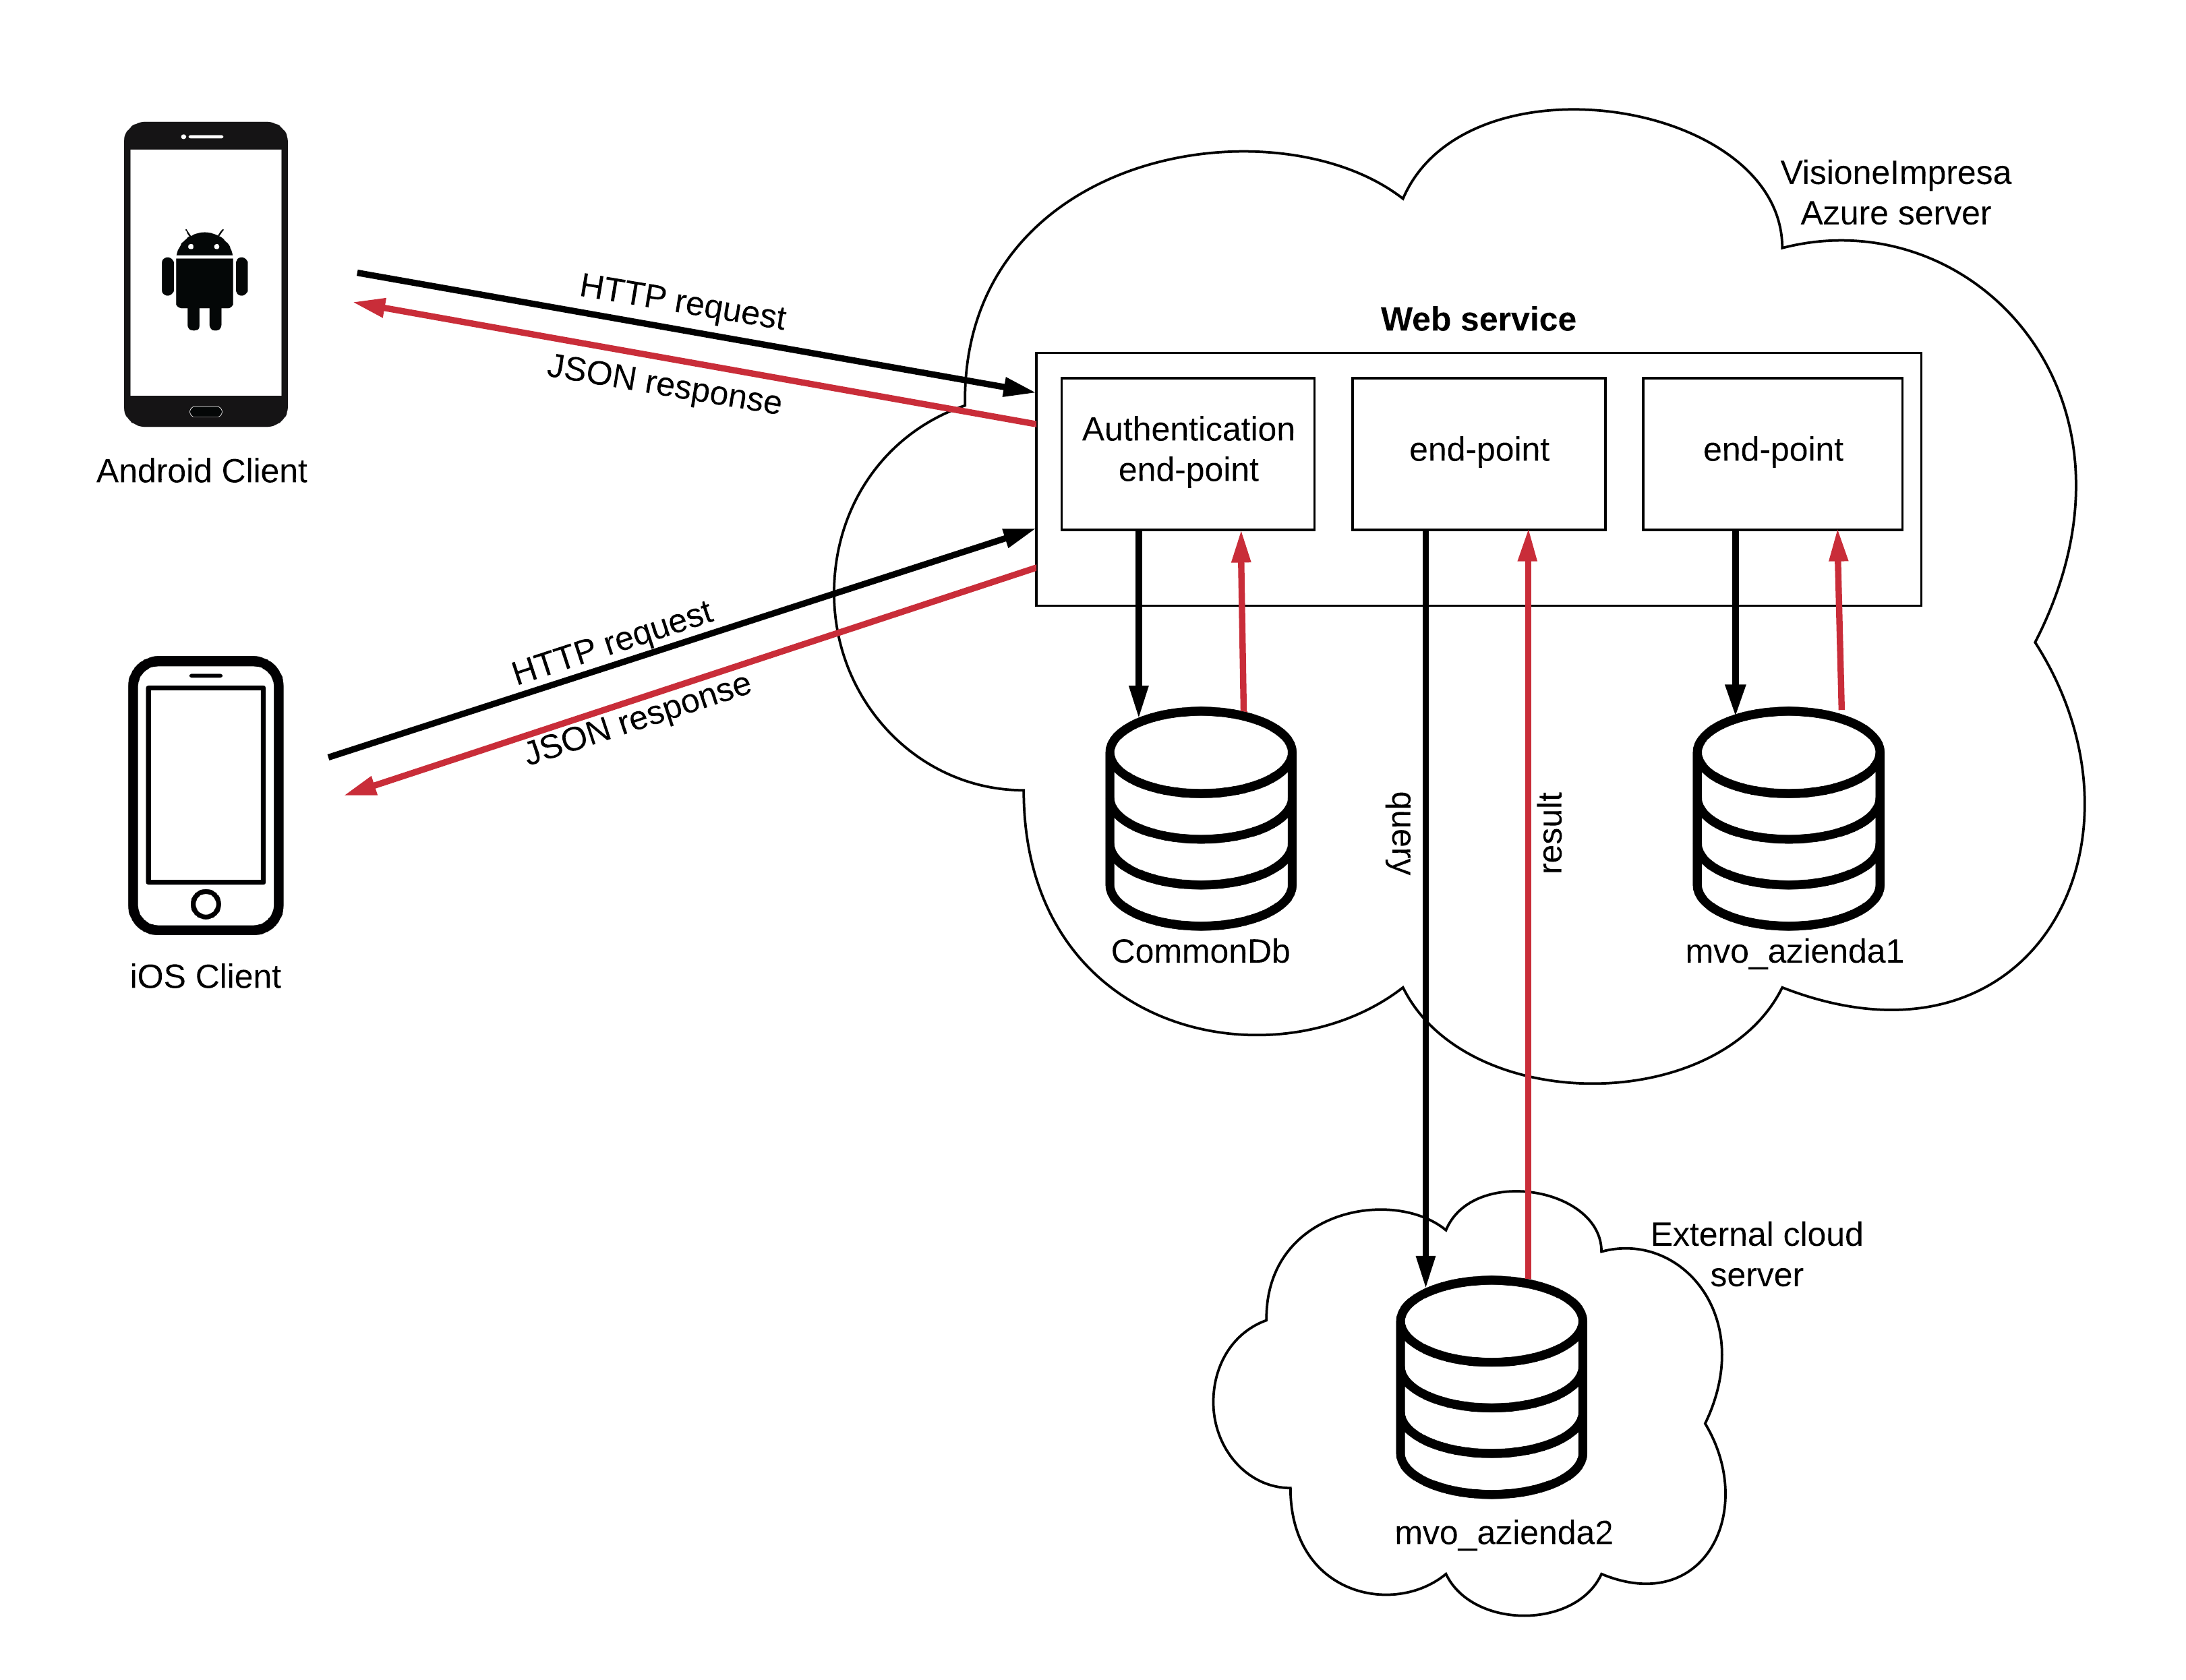
\includegraphics[width=\columnwidth]{progettazione/generalArchitecture} 
    \caption{Architettura generale di moviORDER}
\end{figure}

L'applicazione comunica con il server tramite l'invio di richieste HTTP. Sul server è installato un servizio web che si occupa di elaborare tali richieste tramite oggetti servlet Java, i quali eseguono delle query sul database e rispondono, sulla base dei risultati ottenuti, tramite strighe codificate in formato JSON. Per la costuzione delle risposte, il servizio web interroga i seguenti database SQL Server:
\begin{itemize}
	\item \textit{CommonDb}: database locale al server Azure di \visione{} e contenente i dati di autenticazione degli utenti di moviORDER. Ogni qualvolta che un'azienda acquista il servizio, vengono inserite nel \textit{CommonDb} le credenziali di accesso di tutti gli utenti dell'azienda che desiderano utilizzare l'applicazione;
	\item \textit{mvo\_aziendaNomeAzienda}: database contenente i dati utili alla gestione degli ordini presso l'azienda \textit{NomeAzienda}. All'interno del server Azure è presente un database di questo tipo per ogni azienda che usufruisce del servizio e che ha deciso di affidare la gestione completa dei propri ordini a \visione{}. Per le aziende che preferiscono invece gestire internamente i propri ordini, tale database è contenuto nei server cloud delle rispettive aziende. Ne consegue che il servizio web deve essere in grado di connettersi a database locali o remoti.
\end{itemize}
Una descrizione più approffondita dei dati contenuti in questi database è presente in sezione \ref{progdb}.

\subsection{Architettura front end}

Sul client, ovvero l'applicazione installata sul dispositivo dell'utente utilizzatore, è presente il pattern architetturale MVP (Model View Presenter). Tale pattern presenta componenti distribuite, infatti la view e il presenter si trovano sul dispositivo, mentre il model si trova sul server Azure di \visione{} o sul server cloud di un'azienda cliente. Nello specifico, la view è la GUI dell'applicazione, il presenter è la logica applicativa della stessa e il model è il database contenente i dati utili alla gestione degli ordini. È stato scelto un MVP in quanto il model interagisce solamente con il presenter e non può modificare la view come invece accade per il pattern MVC (Model View Controller). Nella seguente figura è possibile notare le differenze concettuali tra i due pattern.

\begin{figure}[!h] 
    \centering 
    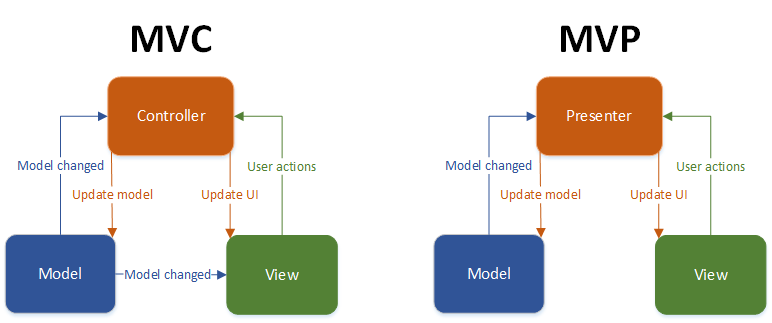
\includegraphics[width=\columnwidth]{progettazione/differenzepattern} 
    \caption{Differenze tra pattern MVC e MVP}
\end{figure}

Viene di seguito presentata una figura illustrativa di come il design pattern MVP è stato istanziato nell'architettura del front end di moviORDER.

\begin{figure}[!h] 
    \centering 
    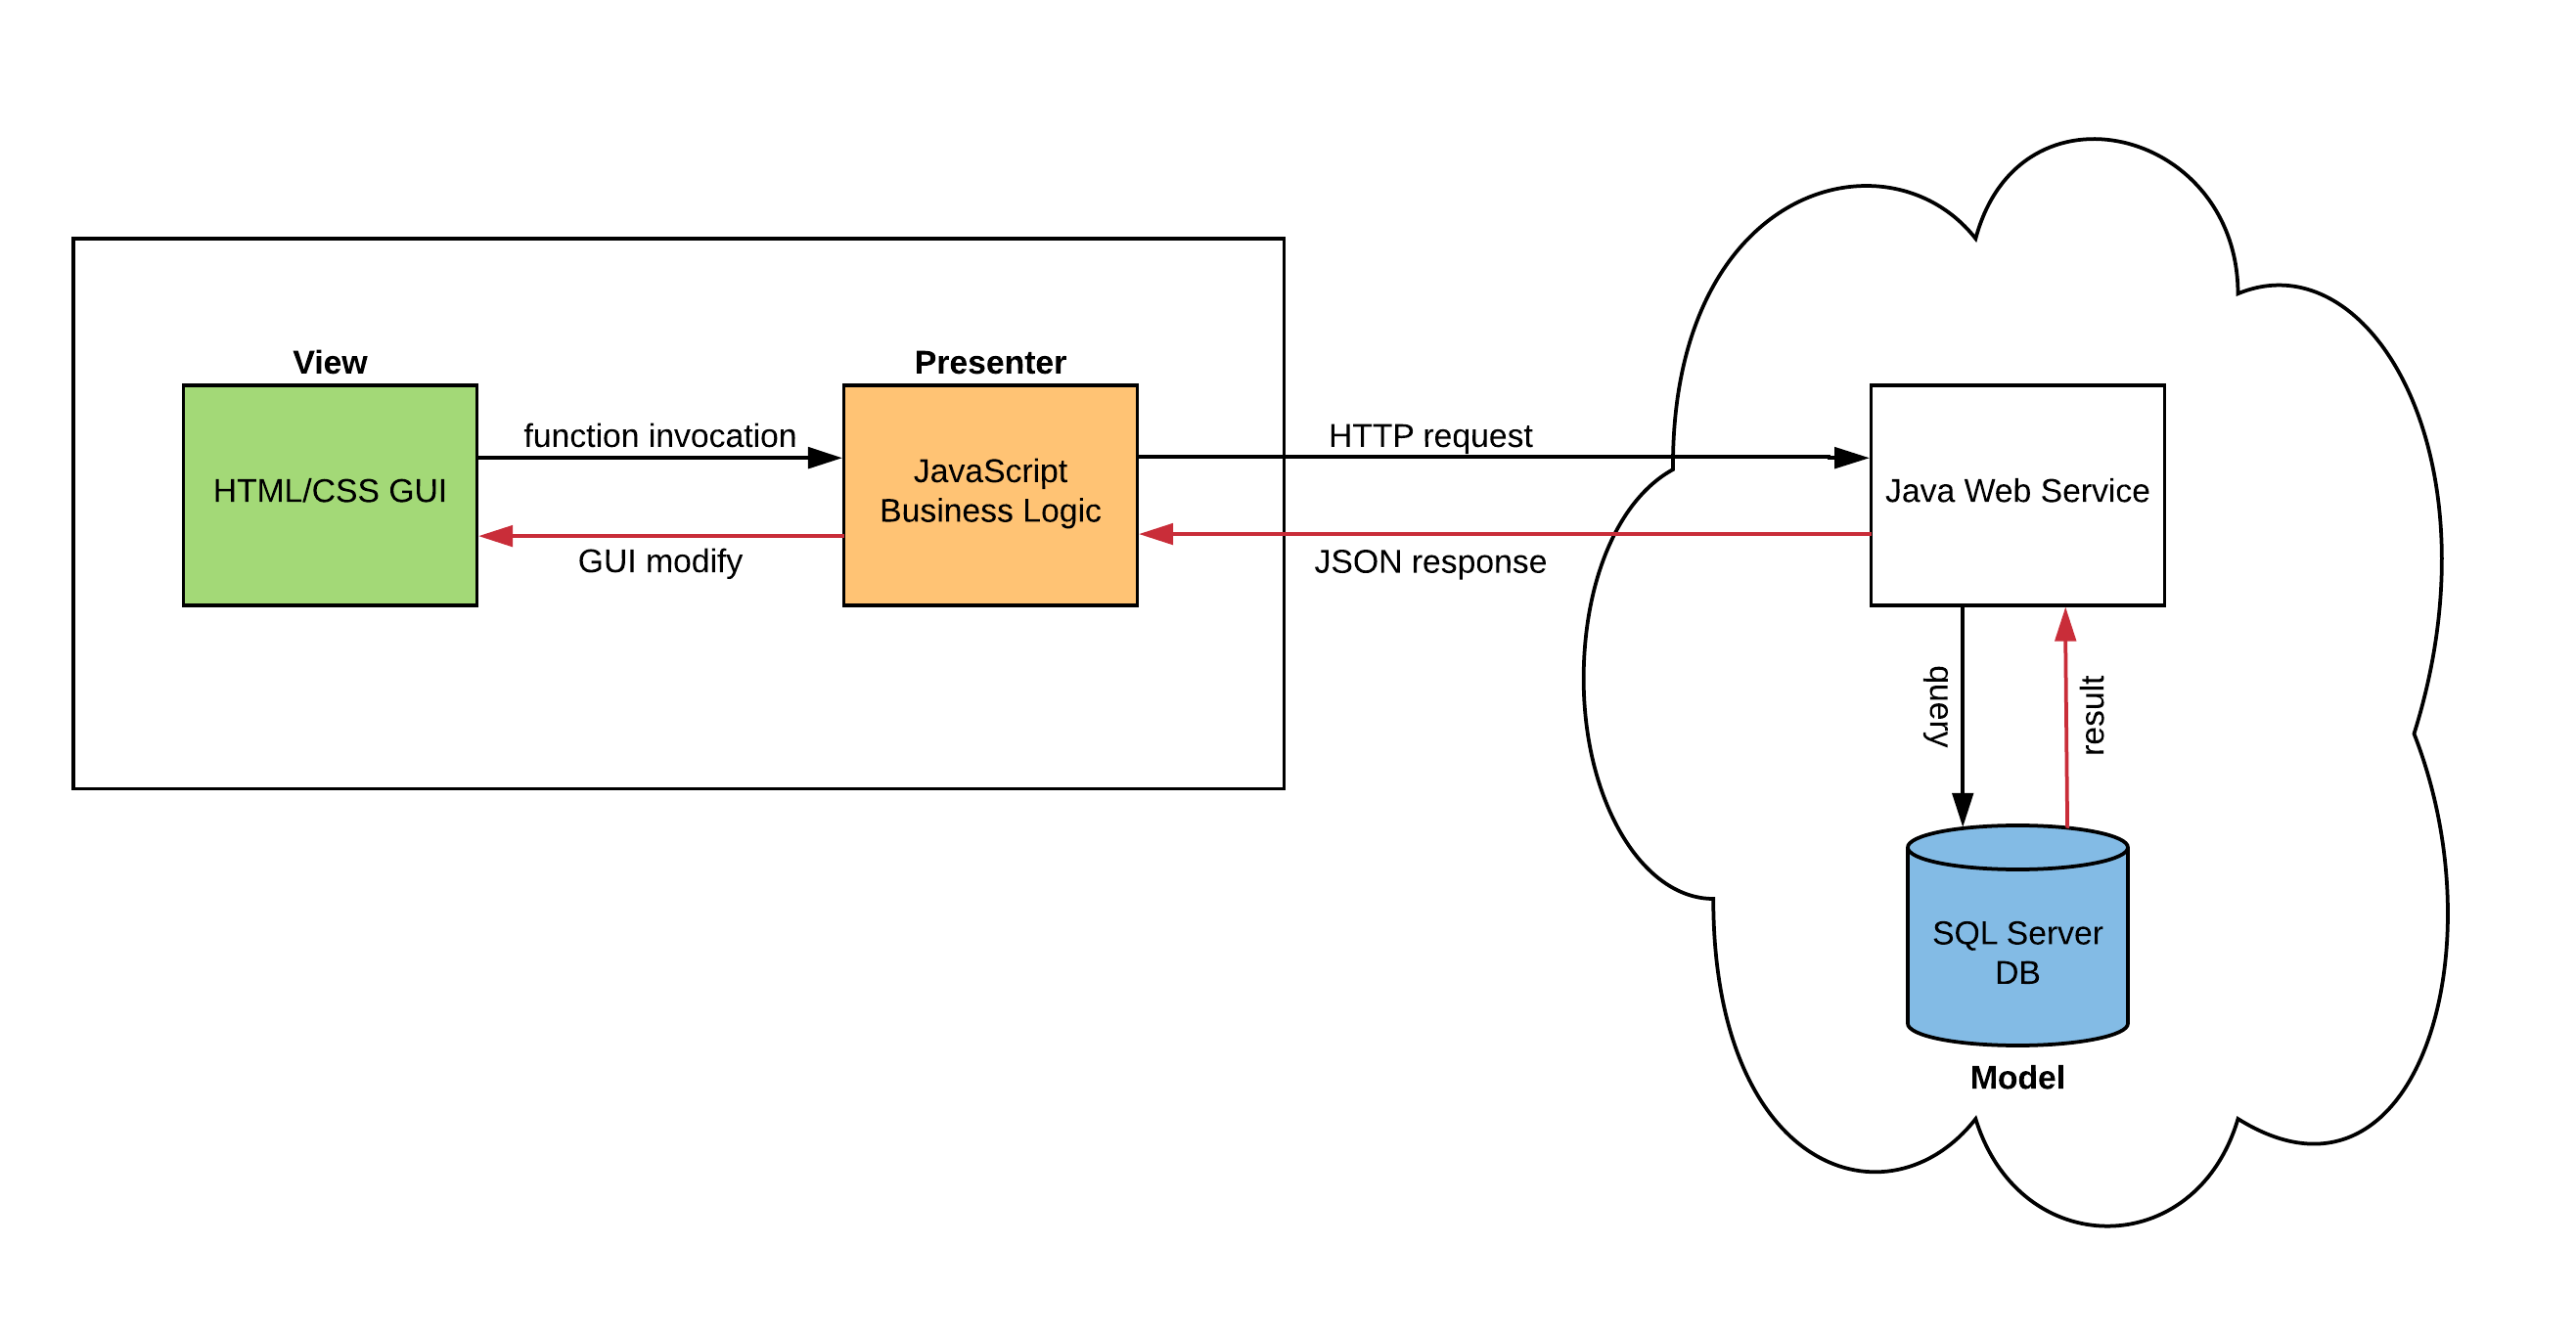
\includegraphics[width=\columnwidth]{progettazione/frontendMVP} 
    \caption{Architettura front end}
\end{figure}

Nello specifico, il flusso del pattern è il seguente:
\begin{itemize}
	\item l'utente interagisce con la view eseguendo delle operazioni sull'interfaccia dell'applicazione;
	\item il presenter capta le interazioni e, sulla base di queste, richiede la lettura/scrittura di dati sul model tramite l'invio di richieste HTTP ad un servizio web;
	\item il servizio web legge/scrive sul model a seconda della richiesta ricevuta e prepara ed invia una risposta al presenter;
	\item il presenter riceve la risposta, la elabora e modifica la view di conseguenza.
\end{itemize}
Viene di seguito presentato un diagramma di sequenza esemplificativo del pattern MVP istanziato nel contesto del progetto.

\begin{figure}[!h] 
    \centering 
    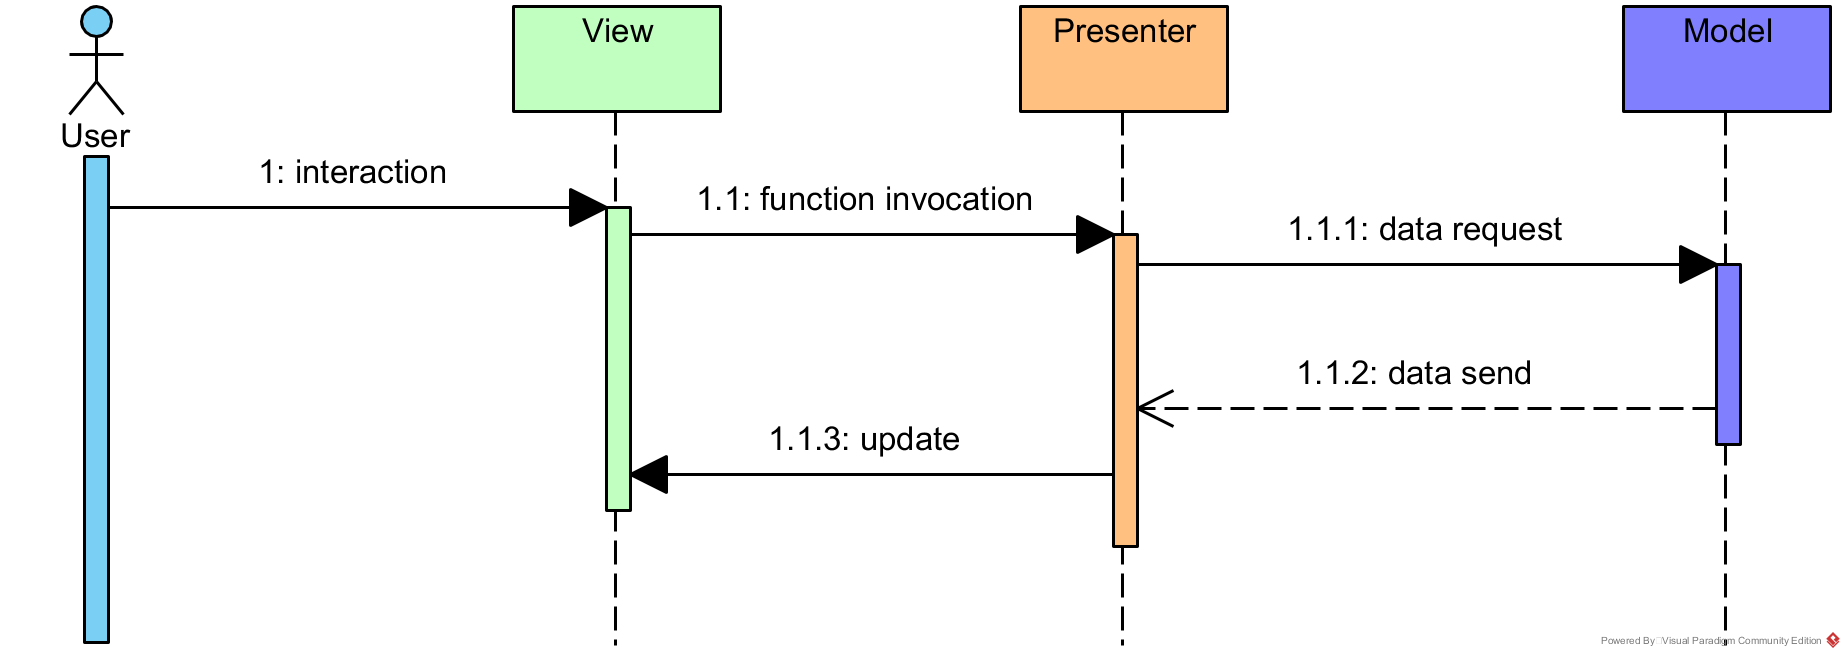
\includegraphics[width=\columnwidth]{progettazione/mvpSequenceDiagram} 
    \caption{Diagramma di sequenza del pattern MVP}
\end{figure}

Importanti vantaggi nell'utilizzo del pattern MVP sono:
\begin{itemize}
	\item possibilità di utilizzare lo stesso model da parte di view differenti;
	\item semplicità nell'aggiunta di nuovi tipi di client, e quindi di applicazioni: è sufficiente scrivere un presenter e una view per ognuna delle nuove applicazioni. MVP permette quindi un disaccoppiamento tra logica applicativa e database sottostante.
\end{itemize}

\subsection{Architettura back end}

Il server presenta un'architettura a strati. In questo pattern i componenti sono organizzati in strati orizzontali e ogni strato possiede specifici ruoli e responsabilità nel contesto dell'applicazione. Nel caso di moviORDER, il pattern è stato diviso nei seguenti strati:
\begin{itemize}
	\item \textbf{business layer}: contiene gli oggetti servlet del servizio web, i quali si occupano di captare le richieste HTTP provenienti dal client, di leggere o scrivere sul database di conseguenza, e di fornire delle risposte;
	\item \textbf{persistance layer}: contiene le classi del servizio web che permettono agli oggetti servlet di accedere al database dell'applicazione;
	\item \textbf{database layer}: contiene i database dell'applicazione.
\end{itemize}
Viene di seguito presentata una figura illustrativa di come il design pattern \textit{layered architecture} è stato istanziato nell'architettura del back end di moviORDER. 

\begin{figure}[!h] 
    \centering 
    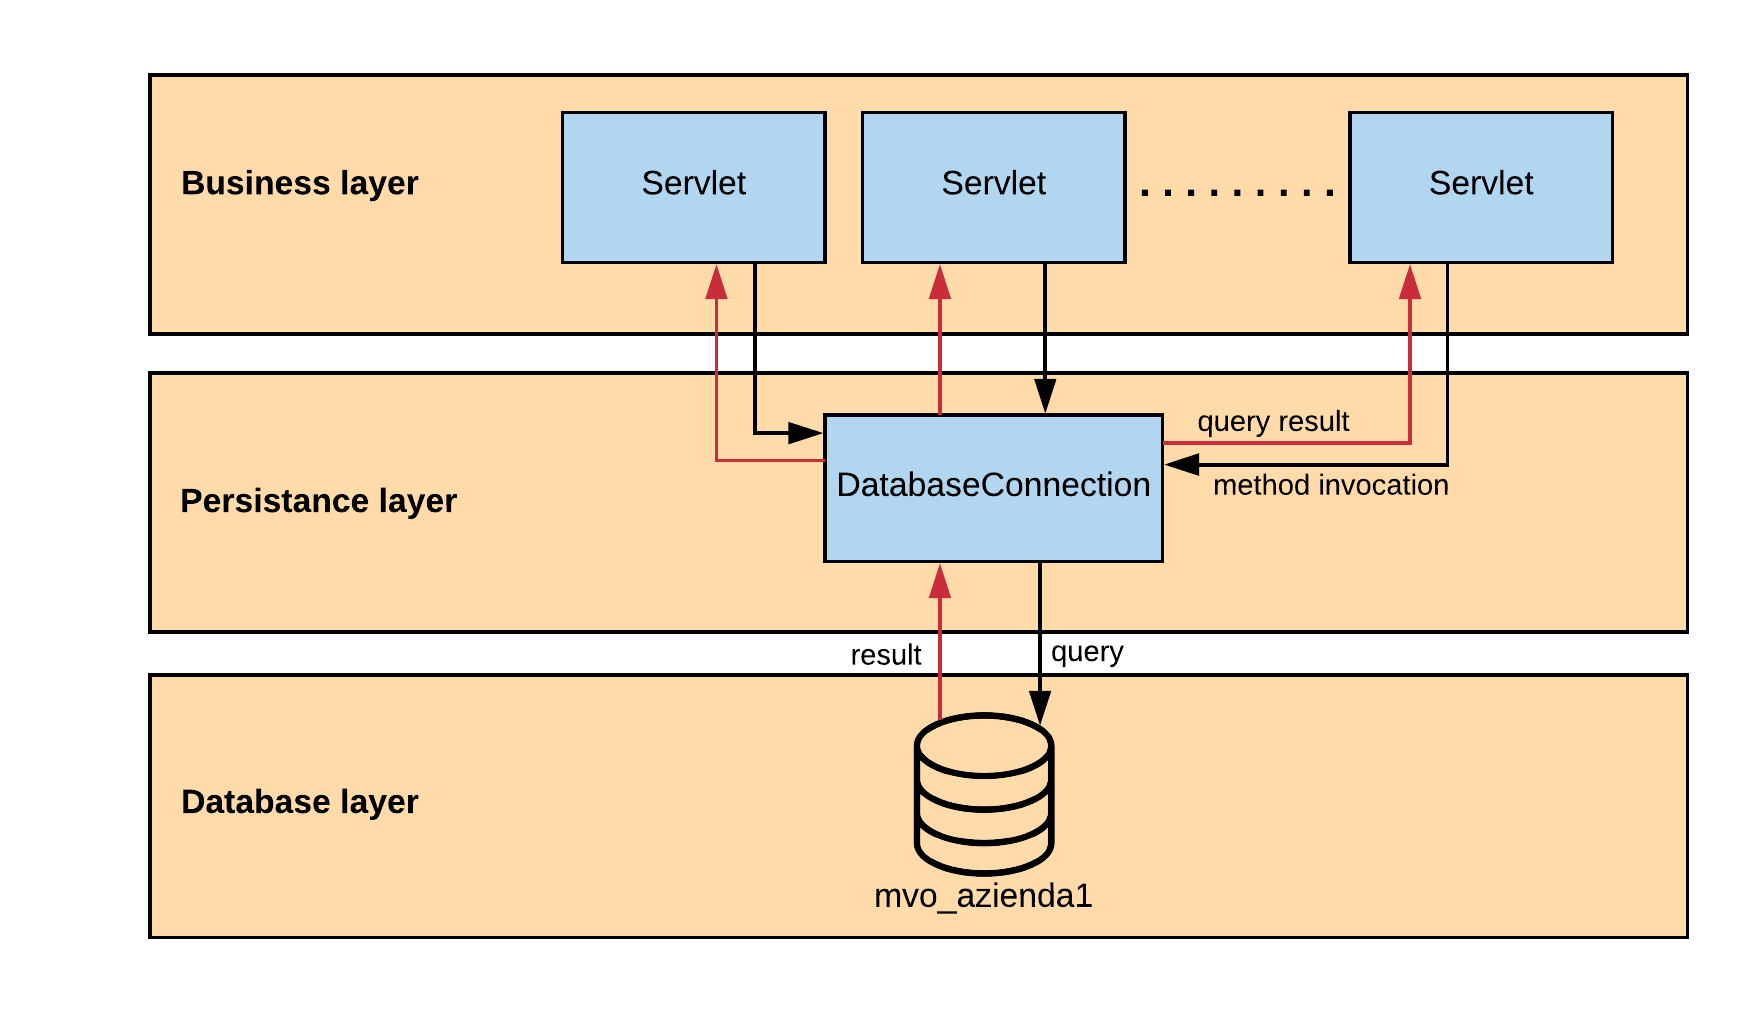
\includegraphics[width=\columnwidth]{progettazione/serverArchitecture} 
    \caption{Architettura a strati del back end}
\end{figure}

Uno dei vantaggi più importanti dell'architettura a strati è la separazione delle responsabilità tra i componenti. Un componente all'interno di uno specifico strato può eseguire solamente compiti che spettano a tale strato. Questo tipo di classificazione facilita lo sviluppo, il testing e la manutenzione del backend di moviORDER.

\section{Progettazione servizio web}

Il seguente diagramma dei package rappresenta la struttura del servizio web di moviORDER.

\begin{figure}[!h] 
    \centering 
    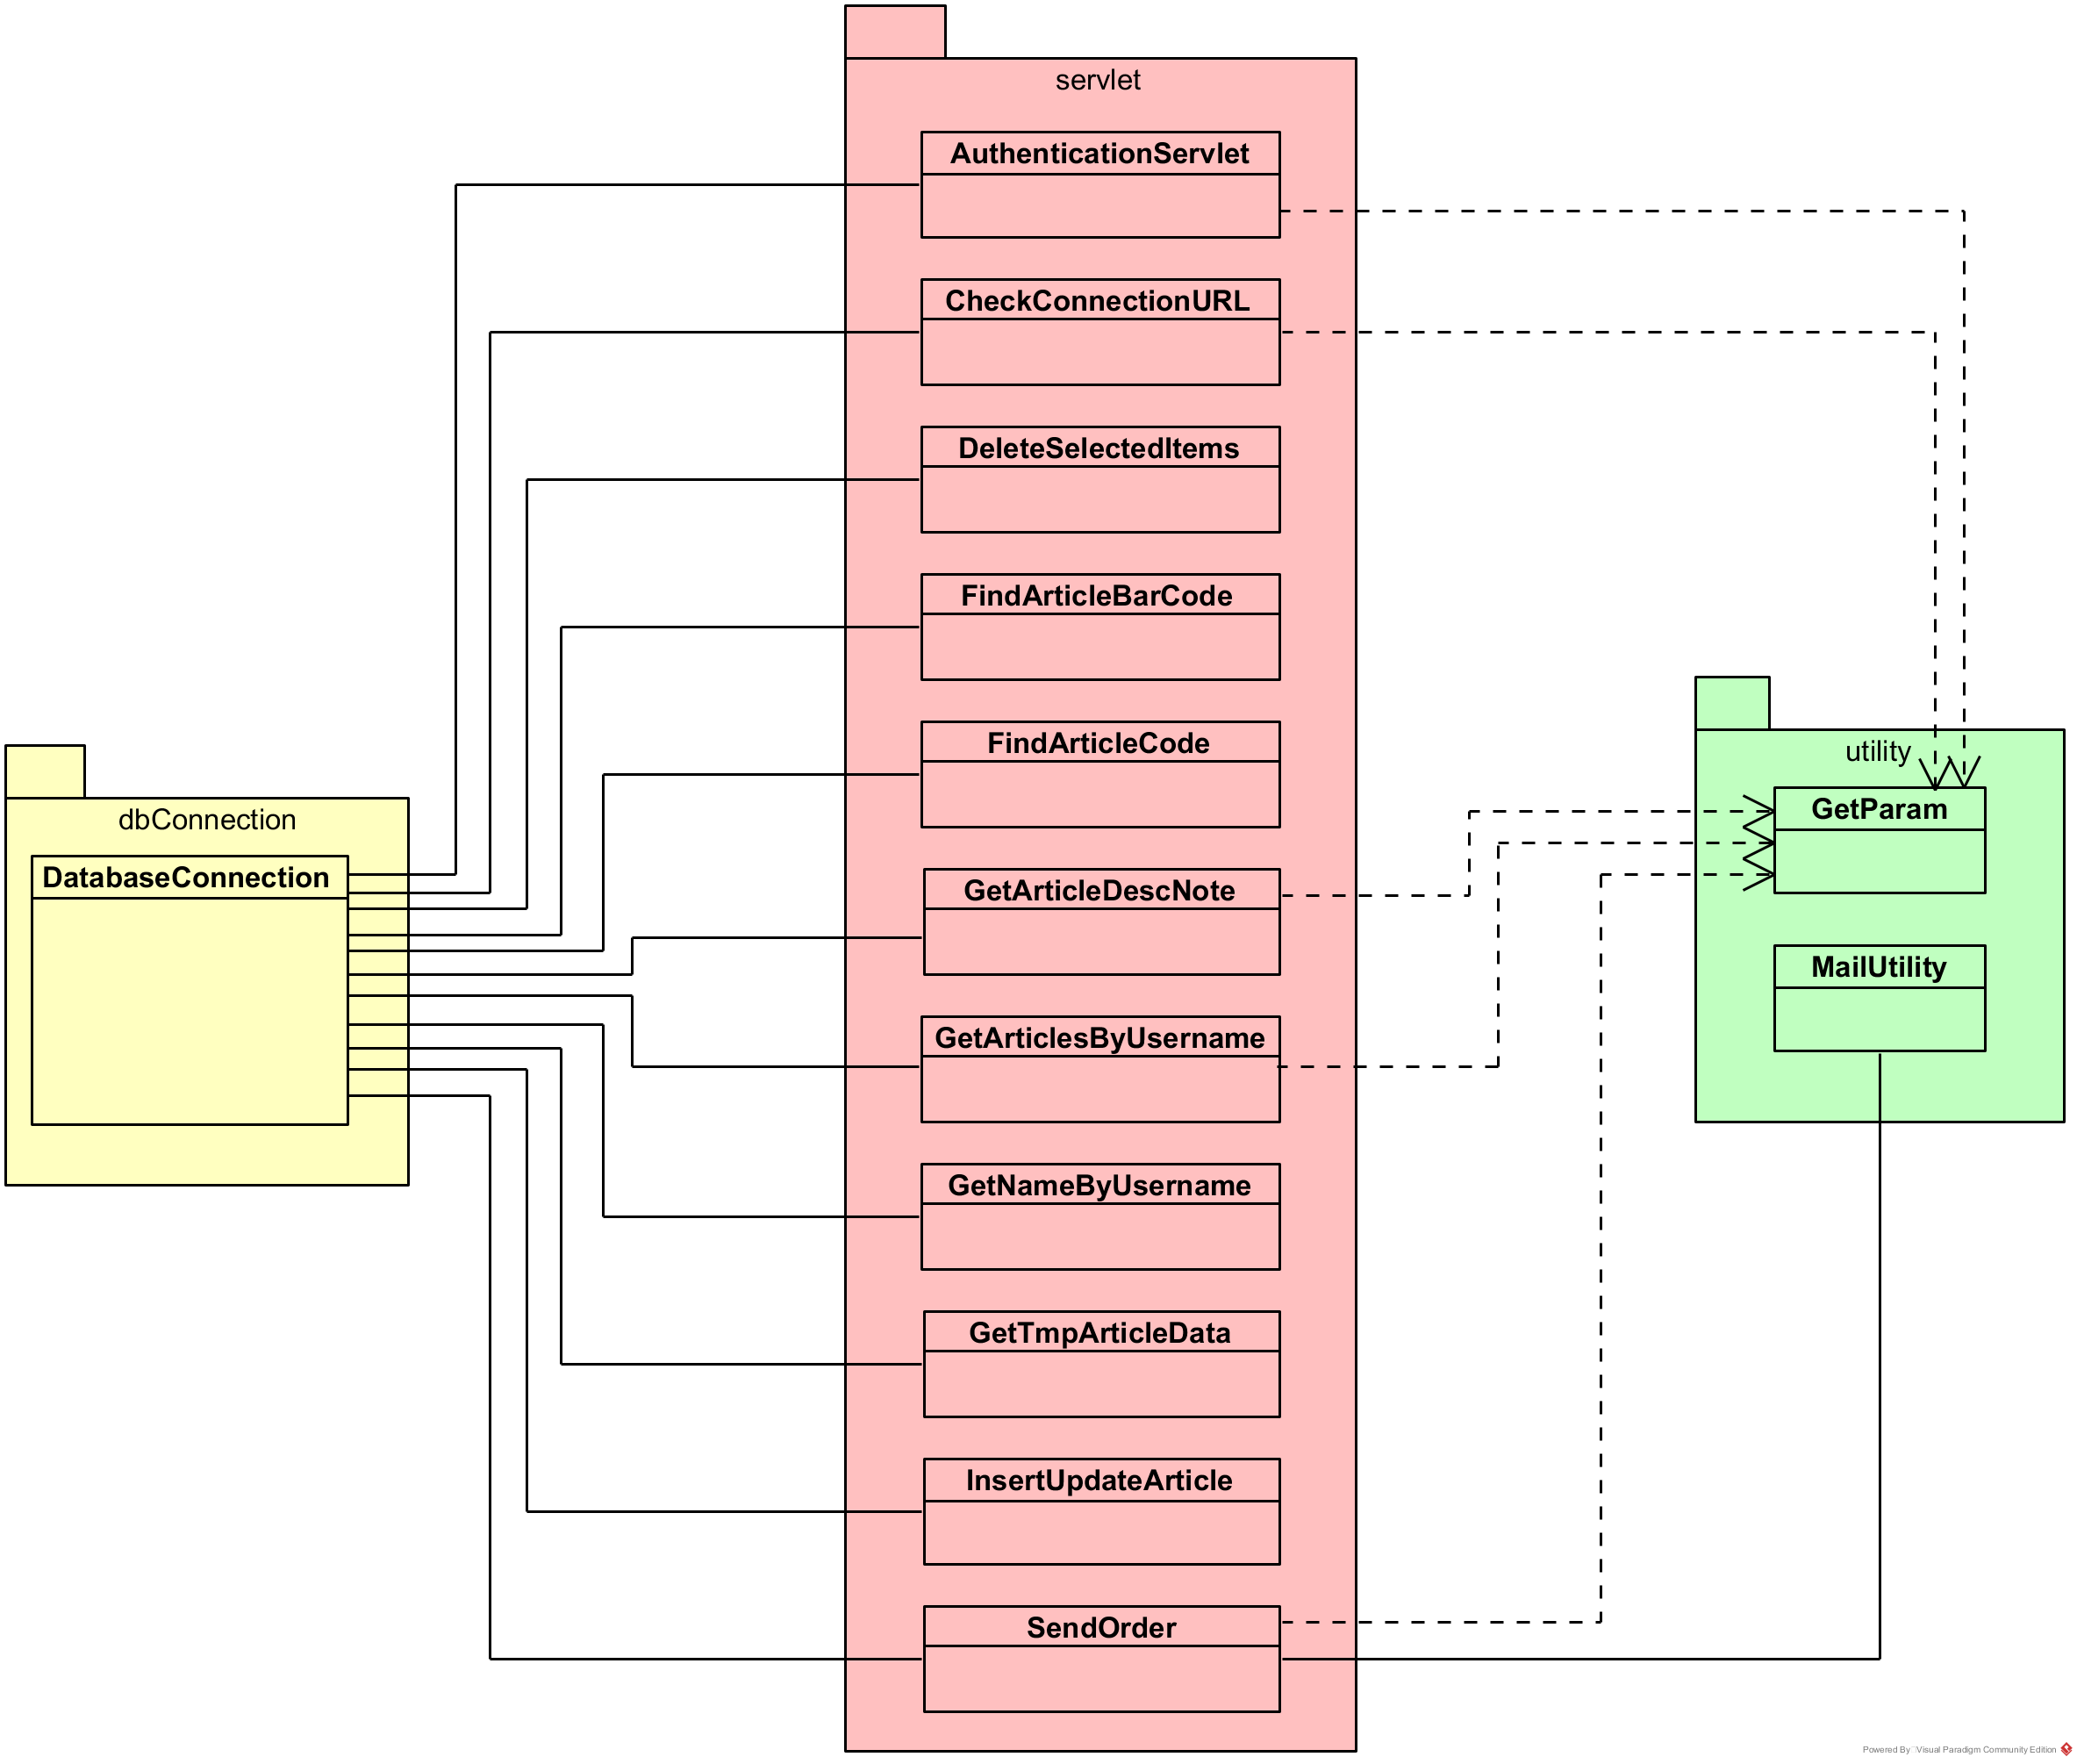
\includegraphics[width=\columnwidth]{progettazione/packages} 
    \caption{Diagramma dei package del servizio web}
\end{figure}

Come si può vedere dal diagramma, il servizio è costituito da tre package:
\begin{itemize}
	\item \textit{dbConnection}: contiene classi atte alla gestione della connessione con un database. Il package viene utilizzato per permettere agli oggetti servlet di connettersi a database SQL Server locali o remoti;
	\item \textit{servlet}: contiene le classi che definiscono gli oggetti servlet del servizio. Questi oggetti si occupano di captare le richieste HTTP provenienti dal client e di rispondere a queste tramite stringhe in formato JSON;
	\item \textit{utility}: contiene le classi utilità del servizio. Queste classi facilitano i compiti che gli oggetti servlet devono eseguire.
\end{itemize}
Una descrizione più appronfondita di come tali package sono stati utilizzati nella codifica del servizio web è presente in sezione \ref{codificaservizio}.

\subsection{Package servlet}

Essendo il package \textit{servlet} il più articolato, merita una descrizione più approfondita. Il seguente diagramma delle classi rappresenta la struttura del package \textit{servlet}.

\begin{figure}[!h] 
    \centering 
    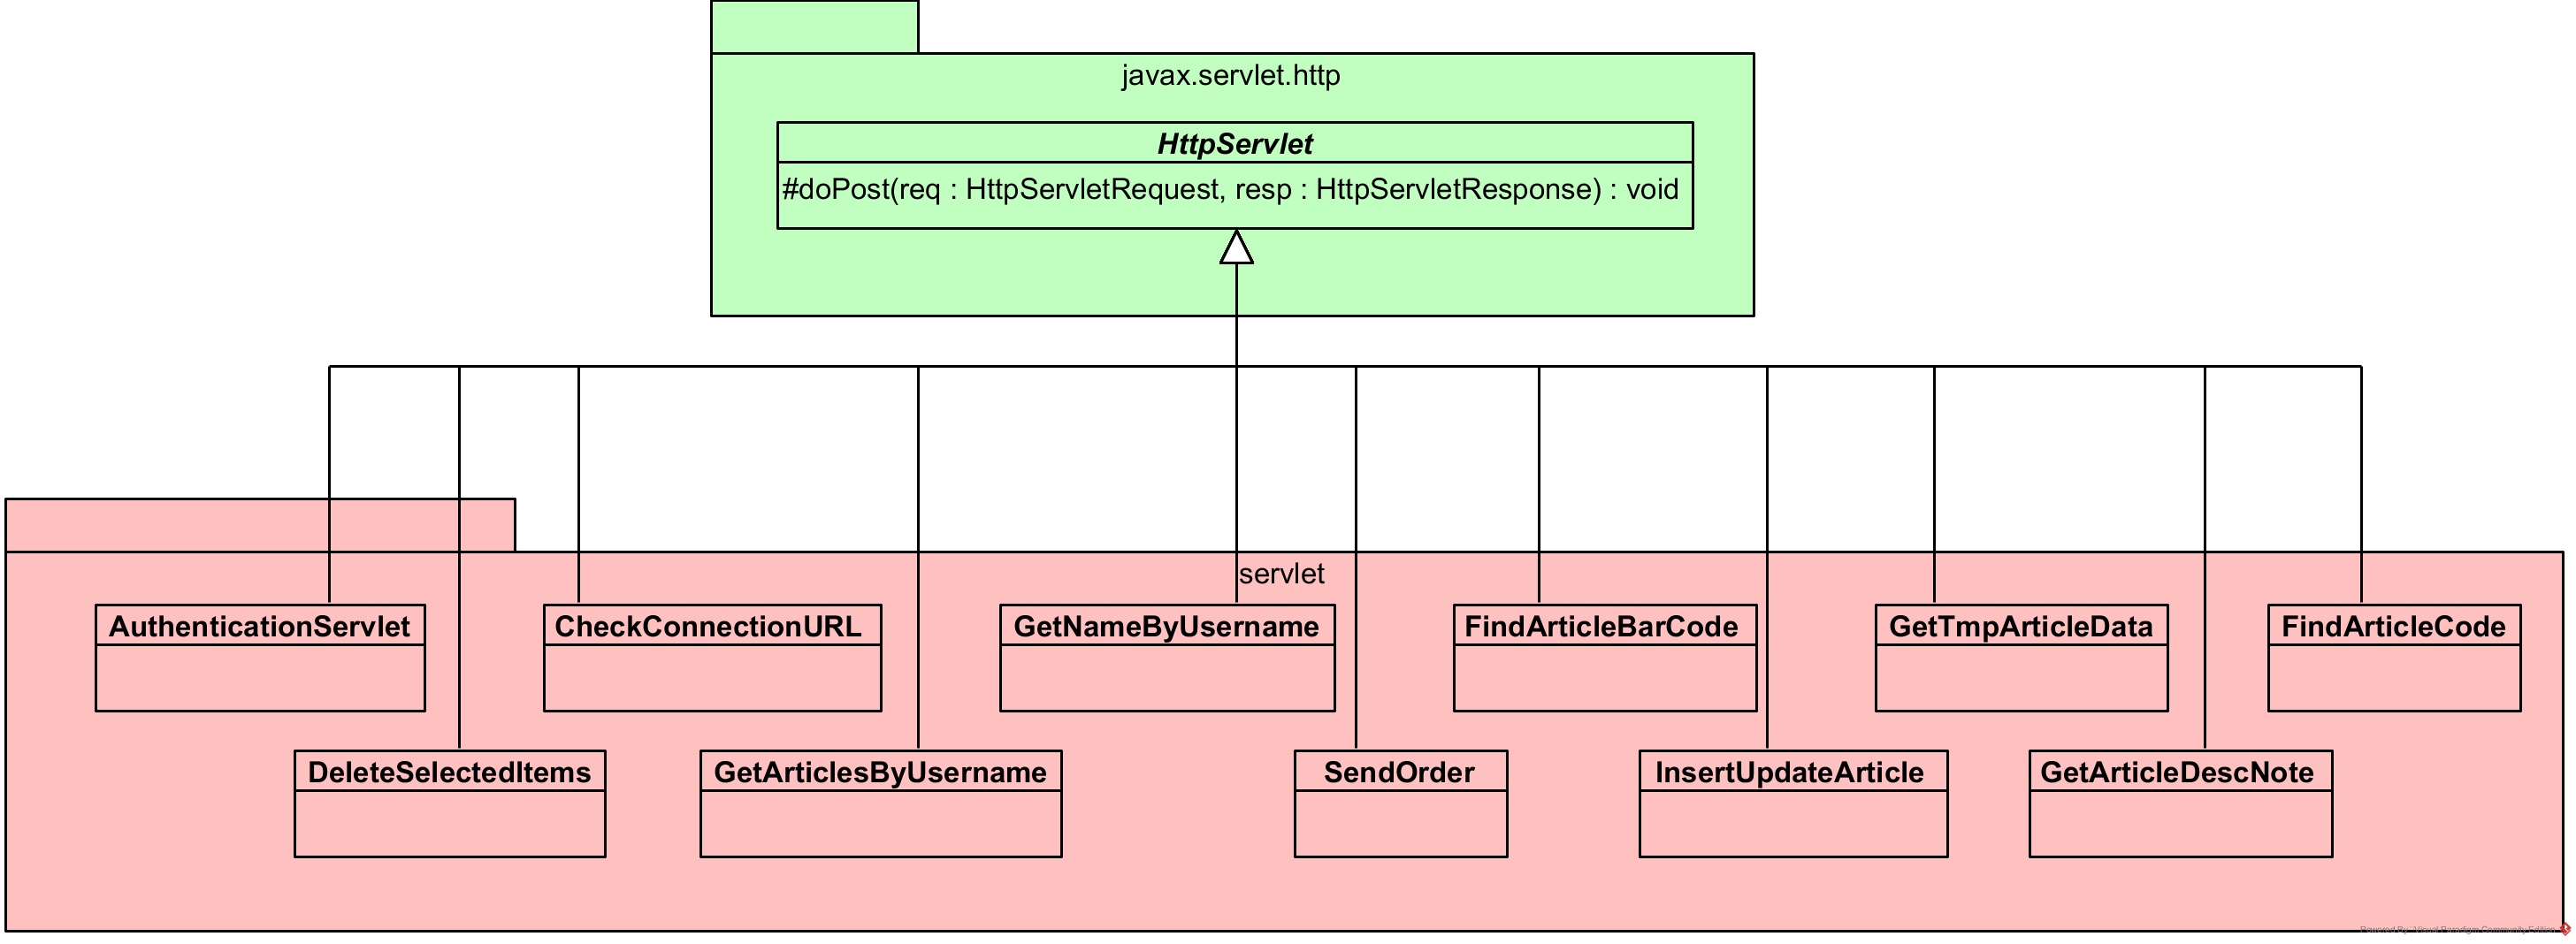
\includegraphics[width=\columnwidth]{progettazione/servletPackage} 
    \caption{Diagramma delle classi del package \textit{servlet}}
\end{figure}

Come si può vedere dal diagramma, ogni classe servlet concreta eredita dalla classe astratta \textit{HttpServlet}. Inoltre, ogni servlet concreto definisce il metodo \textit{doPost()}, il quale permette di definire il comportamento del servlet alla ricezione di richieste HTTP POST. Una descrizione di come queste classi sono state implementate nella pratica è presente in sezione \ref{codificaservizio}.

\section{Progettazione database} \label{progdb}

Come detto precedentemente, i dati di moviORDER sono raggruppati all'interno di due database. Il database \textit{CommonDb} contiene i dati di autenticazione degli utenti di moviORDER e le stringhe di connessione ai rispettivi database aziendali (ogni azienda possiede un proprio database), mentre il database \textit{mvo\_aziendaNomeAzienda} contiene tutti i dati utili alla gestione degli ordini presso l'azienda \textit{NomeAzienda}. Più precisamente, in fase di autenticazione le credenziali dell'utente vengono cercate all'interno del \textit{CommonDb} e, in caso di corrispondenza, viene prelevata la stringa di connessione al database dell'azienda presso cui l'utente è cliente. In seguito questa stringa viene utilizzata per collegare l'applicazione al database corretto e quindi permettere all'utente di visualizzare solamente i dati sugli articoli venduti dalla propria azienda.
Il \textit{CommonDb} presenta le seguenti tabelle:
\begin{itemize}
	\item \textbf{Users}: tabella contenente i dati di autenticazione degli utenti di moviORDER. La tabella presenta i seguenti campi:
		\begin{itemize}
			\item \textit{UserName} (chiave primaria): è il nome utente per accedere all'applicazione. Viene reso univoco poiché costituito dalla concatenazione della partita IVA dell'azienda presso cui l'utente è cliente e un codice auto-incrementante assegnato al cliente al momento della consegna dell'applicazione;
			\item \textit{Password}: è la password per accedere all'applicazione. La coppia username/password viene assegnata all'utente al momento della consegna dell'applicazione;
			\item \textit{CodAzienda} (chiave esterna): è l'identificativo univoco dell'azienda presso cui l'utente è cliente. Questo campo presenta un vincolo d'integrità referenziale con il campo \textit{CodAzienda} della tabella \textbf{Aziende};
			\item \textit{EmailU}: è l'indirizzo e-mail dell'utente;
			\item \textit{Bloccato}: è un flag che vale 1 se l'utente è stato bloccato dall'azienda, oppure 0 se l'utente è operativo e quindi può utilizzare l'applicazione.
		\end{itemize}
	\item \textbf{Aziende}: tabella contenente le stringhe di connessione ai database aziendali di tutte le aziende registrate al servizio moviORDER. Sono presenti inoltre i parametri di configurazione del server SMTP di ogni azienda. Questo server viene utilizzato da moviORDER per inviare le mail di conferma dei vari ordini registrati. La tabella presenta i seguenti campi:
	\begin{itemize}
		\item \textit{CodAzienda} (chiave primaria): è l'identificativo univoco dell'azienda;
		\item \textit{Path}: è la stringa di connessione al database aziendale dell'azienda;
		\item \textit{EmailA}: è l'indirizzo e-mail aziendale dell'azienda;
		\item \textit{Host}: è l'indirizzo della macchina dove è installato il server SMTP dell'azienda;
		\item \textit{Post}: è la porta su cui è installato il server SMTP dell'azienda;
		\item \textit{Username}: è il nome utente per accedere al server SMTP dell'azienda;
		\item \textit{Password}: è la password per accedere al server SMTP dell'azienda.
	\end{itemize}
\end{itemize}
Viene di seguito presentato il diagramma Entity Relationship del database \textit{CommonDb}. Le chiavi primarie sono state sottolineate, mentre le chiavi esterne sono state scritte in corsivo.

\begin{figure}[!h] 
    \centering 
    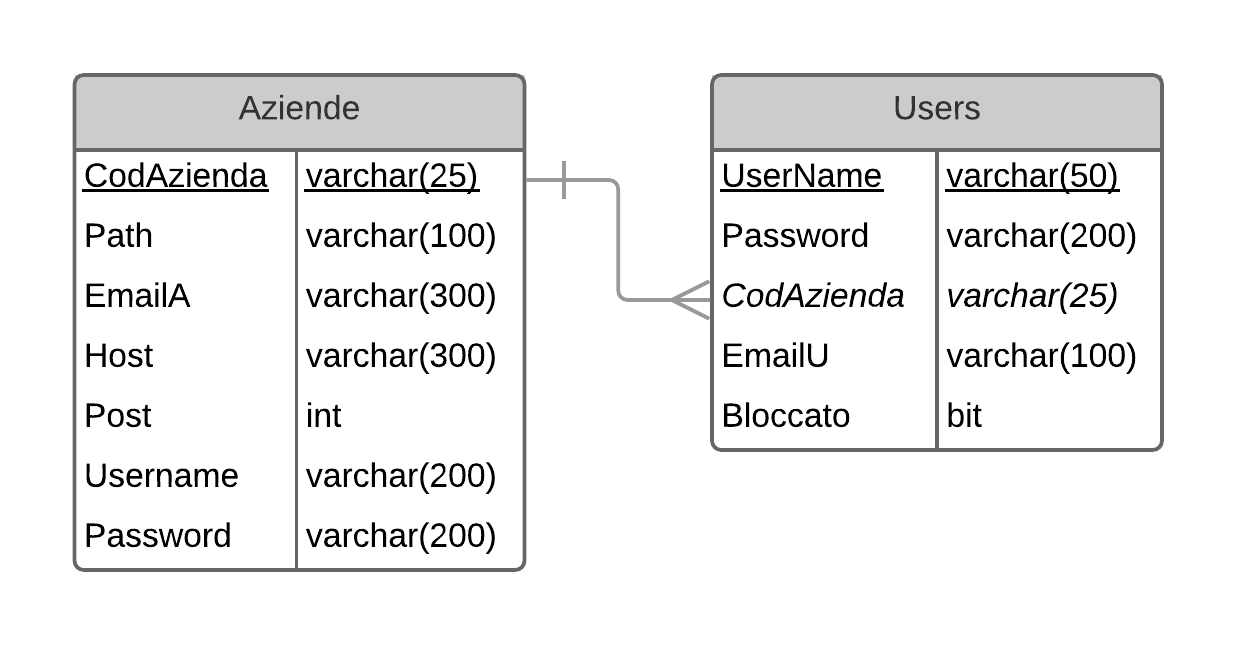
\includegraphics[width=\columnwidth]{progettazione/erCommon} 
    \caption{Diagramma ER di \textit{CommonDb}}
\end{figure}

Il \textit{mvo\_aziendaNomeAzienda} presenta le seguenti tabelle:
\begin{itemize}
	\item \textbf{Art}: tabella contenente i dati sugli articoli venduti dall'azienda \textit{NomeAzienda}. La tabella presenta i seguenti campi:
		\begin{itemize}
			\item \textit{Id\_Art}: è un codice auto-incrementante assegnato al record;
			\item \textit{CodArt} (chiave primaria): è il codice articolo dell'articolo;
			\item \textit{DesArt}: è il nome dell'articolo;
			\item \textit{Note}: sono le note presenti in database per l'articolo;
			\item \textit{QtaMin}: è la minima quantità ordinabile per l'articolo;
			\item \textit{QtaMul}: è lo step di quantità ordinabile per l'articolo. Ad esempio se \textit{QtaMul} è 2, significa che è possibile ordinare 2, 4, 6 pezzi dell'articolo, e così via.
		\end{itemize}
	\item \textbf{ArtAlias}: tabella contenente i codici a barre degli articoli venduti dall'azienda. La tabella presenta i seguenti campi:
		\begin{itemize}
			\item \textit{Id\_ArtAlias}: è un codice auto-incrementante assegnato al record;
			\item \textit{CodArt} (chiave primaria, chiave esterna): è il codice articolo dell'articolo. Questo codice presenta un vincolo d'integrità referenziale con il campo \textit{CodArt} della tabella \textbf{Art};
			\item \textit{Alias} (chiave primaria): è il codice a barre dell'articolo. Fa parte della chiave primaria, insieme a \textit{CodArt}, poiché è possibile che un articolo abbia più codici a barre.
		\end{itemize}
	\item \textbf{DocRig}: tabella contenente i dati d'ordine degli articoli che sono stati ordinati presso l'azienda. La tabella presenta i seguenti campi:
		\begin{itemize}
			\item \textit{Id\_DocRig} (chiave primaria): è un codice auto-incrementante assegnato al record; 
			\item \textit{Id\_DocTes} (chiave esterna): è il codice della fattura a cui il prodotto ordinato appartiene. Questo campo presenta un vincolo di integrità referenziale con il campo \textit{Id\_DocTes} della tabella \textbf{DocTes};
			\item \textit{Username} (chiave esterna): è il nome utente dell'utente che ha ordinato l'articolo. Questo campo presenta un vincolo d'integrità referenziale con il campo \textit{UserID} della tabella \textbf{Users};
			\item \textit{CodArt} (chiave esterna): è il codice articolo dell'articolo ordinato. Questo campo presenta un vincolo d'integrità referenziale con il campo \textit{CodArt} della tabella \textbf{Art};
			\item \textit{Quantita}: è la quantità ordinata dell'articolo;
			\item \textit{Note}: sono le note che l'utente ha inserito per l'articolo quando l'ha aggiunto al carrello.
		\end{itemize}
	\item \textbf{DocTes}: tabella contenente i dati delle fatture degli ordini che sono stati registrati prezzo l'azienda. La tabella presenta i seguenti campi:
		\begin{itemize}
			\item \textit{Id\_DocTes} (chiave primaria): è un codice auto-incrementante assegnato al record;
			\item \textit{CodDoc} (chiave esterna): è un codice che rappresenta la tipologia di fattura emessa dall'azienda. Questo campo presenta un vincolo d'integrità referenziale con il campo \textit{CodDoc} della tabella \textbf{Users};
			\item \textit{CodCliFor}: è il nome utente dell'utente che ha eseguito l'ordine presso l'azienda;
			\item \textit{DataDoc}: è la data dell'ordine;
			\item \textit{Note}: sono le note inserite dall'utente in fase di invio ordine;
			\item \textit{Status}: è un flag che vale 0 nel momento in cui il record viene memorizzato in tabella, 1 nel momento in cui inizia l'importazione del record nel gestionale di \visione{} e 2 quando l'importazione è terminata.
		\end{itemize}
	\item \textbf{TmpRig}: tabella contenente i dati d'ordine degli articoli non ancora ordinati presso l'azienda. Si tratta di articoli inseriti nel carrello degli utenti, ma che non sono ancora stati ordinati. La tabella presenta i seguenti campi:
		\begin{itemize}
			\item \textit{Id\_TmpRig} (chiave primaria): è un codice auto-incrementante assegnato al record;
			\item \textit{Username} (chiave esterna): è il nome utente dell'utente che presenta l'articolo in carrello. Questo campo presenta un vincolo d'integrità referenziale con il campo \textit{UserID} della tabella \textbf{Users};
			\item \textit{CodArt} (chiave esterna): è il codice articolo dell'articolo. Questo campo presenta un vincolo d'integrità referenziale con il campo \textit{CodArt} della tabella \textbf{Art};
			\item \textit{Quantita}: è la quantità da ordinare inserita dall'utente;
			\item \textit{Note}: sono le note che l'utente ha inserito per l'articolo quando l'ha aggiunto al carrello.
		\end{itemize}
	\item \textbf{Users}: tabella contenente le informazioni anagrafiche degli utenti clienti dell'azienda. La tabella presenta i seguenti campi:
		\begin{itemize}
			\item \textit{UserID} (chiave primaria): è il nome utente dell'utente;
			\item \textit{DesCliFor}: è una breve descrizione dell'utente;
			\item \textit{Indirizzo}: è l'indirizzo di residenza dell'utente;
			\item \textit{Localita}: è la località di residenza dell'utente;
			\item \textit{CodProv}: è il codice della provincia di residenza dell'utente;
			\item \textit{CodNazione}: è il codice della nazione di residenza dell'utente;
			\item \textit{CodDoc}: è il codice della fattura che deve essere emessa quando l'utente effettua un ordine;
			\item \textit{DesDoc}: è una descrizione della fattura che deve essere emessa quando l'utente effettua un ordine.
		\end{itemize}
\end{itemize}
Viene di seguito presentato il diagramma Entity Relationship del database \textit{mvo\_aziendaNomeAzienda}. Le chiavi primarie sono state sottolineate, mentre le chiavi esterne sono state scritte in corsivo.

\begin{figure}[!h] 
    \centering 
    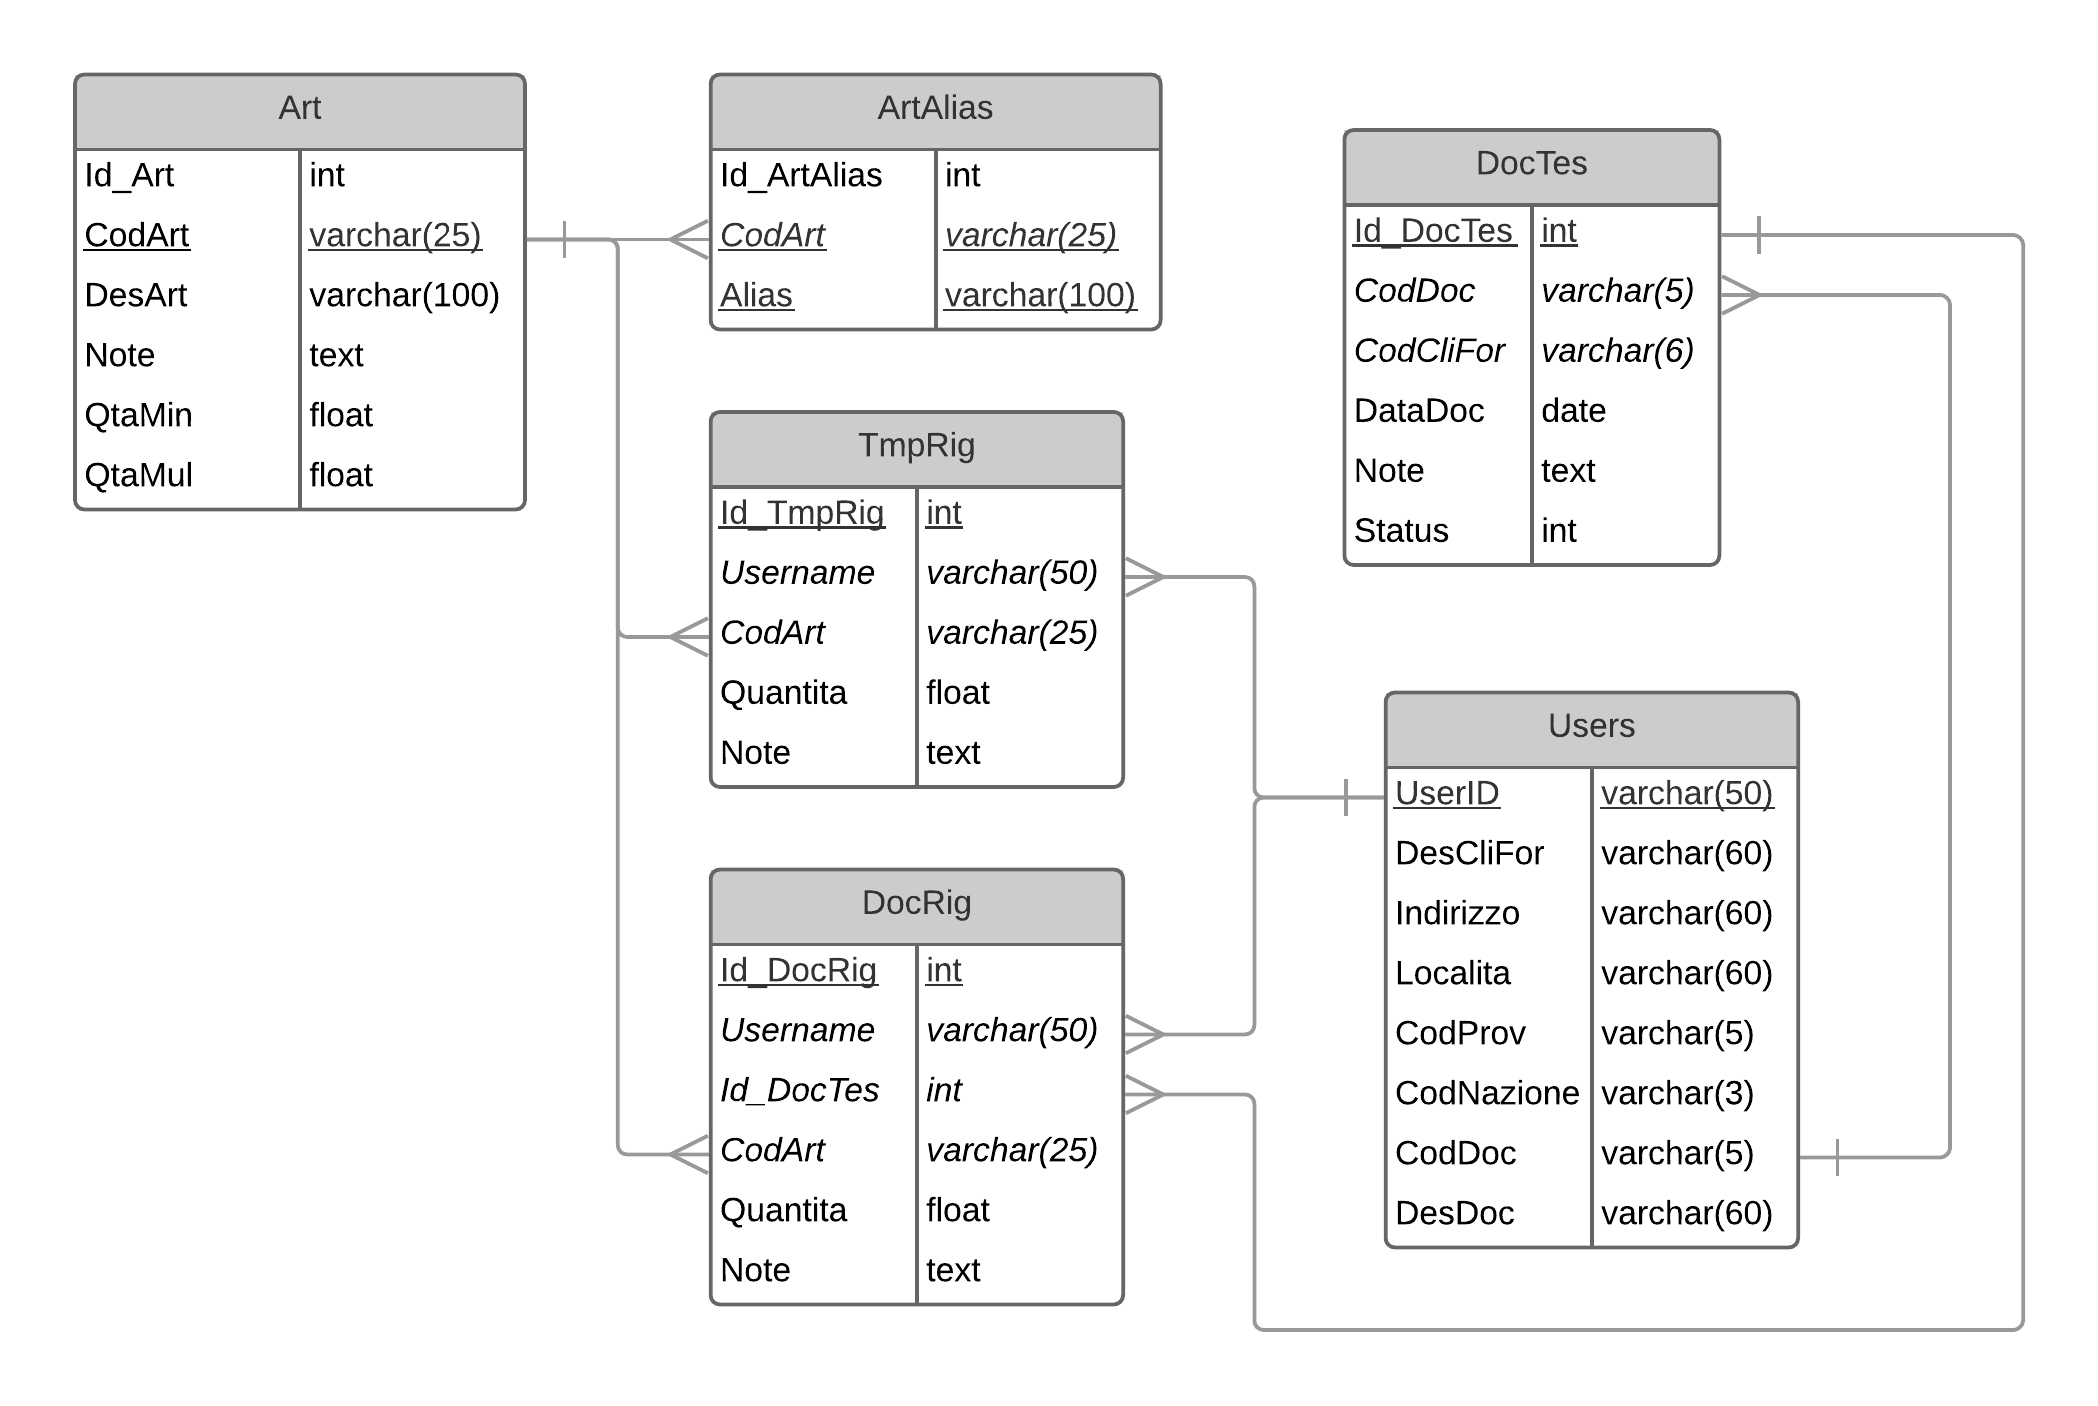
\includegraphics[width=\columnwidth]{progettazione/erMvoAzienda} 
    \caption{Diagramma ER di \textit{mvo\_aziendaNomeAzienda}}
\end{figure}

